
% example for dissertation.sty
\documentclass[
  % Replace oneside by twoside if you are printing your thesis on both sides
  % of the paper, leave as is for single sided prints or for viewing on screen.
  oneside,
  %twoside,
  11pt, a4paper,
  footinclude=true,
  headinclude=true,
  cleardoublepage=empty
]{scrbook}

\usepackage{dissertation}
\usepackage[utf8]{inputenc} %Needed for PT letters unavailable to EN language ( ç,....)

\usepackage{listings}
%LISTING - GENERAL
\lstset{
	basicstyle=\small,
	numbers=left,
	numberstyle=\tiny,
	numbersep=5pt,
	breaklines=true,
	stepnumber=1,
    	frame=tB,
	%mathescape=true,
	escapeinside={(*@}{@*)}
}
%
%\lstset{ %
%	language=Java,							% choose the language of the code
%	basicstyle=\ttfamily\footnotesize,		% the size of the fonts that are used for the code
%	keywordstyle=\bfseries,					% set the keyword style
%	%numbers=left,							% where to put the line-numbers
%	numberstyle=\scriptsize,				% the size of the fonts that are used for the line-numbers
%	stepnumber=2,							% the step between two line-numbers. If it's 1 each line
%											% will be numbered
%	numbersep=5pt,							% how far the line-numbers are from the code
%	backgroundcolor=\color{white},			% choose the background color. You must add \usepackage{color}
%	showspaces=false,						% show spaces adding particular underscores
%	showstringspaces=false,					% underline spaces within strings
%	showtabs=false,							% show tabs within strings adding particular underscores
%	frame=none,								% adds a frame around the code
%	%abovecaptionskip=-.8em,
%	%belowcaptionskip=.7em,
%	tabsize=2,								% sets default tabsize to 2 spaces
%	captionpos=b,							% sets the caption-position to bottom
%	breaklines=true,						% sets automatic line breaking
%	breakatwhitespace=false,				% sets if automatic breaks should only happen at whitespace
%	title=\lstname,							% show the filename of files included with \lstinputlisting;
%											% also try caption instead of title
%	escapeinside={\%*}{*)},					% if you want to add a comment within your code
%	morekeywords={*,...}					% if you want to add more keywords to the set
%}

% ACRONYMS -----------------------------------------------------

%import the necessary package with some options
\usepackage[acronym,nonumberlist,nomain]{glossaries}

%enable the following to avoid links from the acronym usage to the list
%\glsdisablehyper

%displays the first use of an acronym in italic
\defglsdisplayfirst[\acronymtype]{\emph{#1#4}}

%the style of the Glossary
\glossarystyle{listgroup}

% set the name for the acronym entries page
\renewcommand{\glossaryname}{Acronyms}

%this shall be the last thing in the acronym configuration!!
\makeglossaries


% here are the acronym entries
\newacronym{mei}{MEI}{Mestrado em Engenharia Informática}
\newacronym{di}{DI}{Departamento de Informática}
\newacronym{um}{UM}{Universidade do Minho}

\newacronym{qos}{QoS}{Quality of Service}
\newacronym{soa}{SOA}{Service Oriented Architecture}

% these could go in an acronyms.tex file, and loaded with:
% \loadglsentries[\acronymtype]{Parts/Definitions/acronyms}
% when using this, you may want to remove 'nomain' from the package options

%% **MORE INFO** %%

%to add the acronyms list add the following where you want to print it:
%\printglossary[type=\acronymtype]
%\clearpage
%\thispagestyle{empty}

%to use an acronym:
%\gls{qps}

% compile the thesis in command line with the following command sequence:
% pdlatex dissertation.tex
% makeglossaries dissertation
% bibtex dissertation
% pdlatex dissertation.tex
% pdlatex dissertation.tex

% ----------------------------------------------------------------

% Title
\titleA{Implementing a Syntax Directed Editor}
\titleB{for LISS.} % (if any)
%\titleB{for LogoLISS with incremental compilation} % (if any)
%\subtitleA{First Part of Subtitle}
%\subtitleB{Second part of Subtitle} % (if any)

% Author
\author{Damien da Silva Vaz}

% Supervisor(s)
\supervisor{Professor Pedro Rangel Henriques}
\cosupervisor{Professor Daniela da Cruz}

% University (uncomment if you need to change default values)
% \def\school{Escola de Engenharia}
% \def\department{Departamento de Inform\'{a}tica}
% \def\university{Universidade do Minho}
% \def\masterdegree{Computer Science}

% Date
\date{\myear} % change to text if date is not today

% Keywords
%\keywords{master thesis}

% Glossaries & Acronyms
%\makeglossaries  %  either use this ...
%\makeindex	   % ... or this

% Define Acronyms
%%!TEX root = ../dissertation.tex

\newacronym{mei}{MEI}{Mestrado em Engenharia Inform\'{a}tica}
\newacronym{um}{UM}{Universidade do Minho}
%\glsaddall[types={\acronymtype}]



\ummetadata % add metadata to the document (author, publisher, ...)

\begin{document}
	% Cover page ---------------------------------------
	\umfrontcover	
	\umtitlepage
	
	% Add acknowledgements ----------------------------
	\chapter*{Acknowledgements}
	Firstly, I would like to thank my supervisor Pedro Rangel Henriques and co-supervisor Daniela da Cruz. They are the most who supported me throw this ambitious project and took me to the final stage of my university career.\newline
Thank you also to my family and friends (Ranim, Bruno, Chloé, Tiago, Tamara) for supporting me.\newline
And last but not least, I would like to dedicate this thesis to my, particularly, most beautiful mother.
Despite you couldn't be here to watch me conclude my studies. Wherever you are, I hope that you are proud of me.	
None of this could have been made without their unconditional help.

	% Add abstracts (en,pt) ---------------------------
	\chapter*{Abstract}
	The aim of this master work is to implement LISS language in ANTLR compiler generator system using an attribute grammar which create an abstract syntax tree (AST) and generate MIPS assembly code for MARS (MIPS Assembler and Runtime Simulator) .
Using that AST, it is possible to create a Syntax Directed Editor (SDE) in order to provide the typical help of a structured editor which controls the writing according to language syntax as defined by the underlying context free grammar.
	
	\cleardoublepage
	\chapter*{Resumo}
	O tema desta dissertação é implementar a linguagem LISS em ANTLR com um gramática de atributos e no qual, irá criar uma árvore sintática abstrata e gerar MIPS assembly código para MARS (MIPS Assembler and Runtime Simulator).
        Usando esta árvore sintática abstrata, criaremos uma SDE (Editor Dirigido a Sintaxe) no qual fornecerá toda a ajuda típica de um editor estruturado que controlará a escrita de acordo com a gramática.	
	
	% Summary Lists ------------------------------------
	\tableofcontents
	\listoffigures
	\listoftables
	%\lstlistoflistings
	%\listofabbreviations
	\printglossary[type=\acronymtype]
	\clearpage
	\thispagestyle{empty}

	
	\pagenumbering{arabic}
	
	% CHAPTER - Introduction -------------------------
	\chapter{Introduction}
In informatics, solving problems with computers is related to the necessity of helping the end-users, facilitating their life.
And all these necessities pass through developers who creates programs for this purpose.

However, developing programs is a difficult task; analyzing problems, and debugging software takes effort and time.

And this is why we must find a solution for these problems.

Developing a software package  requires tools to help the developers to maximize their programming productivity.
These tools are: on one hand, compilers to generate lower-level code (machine code) from the high-level source code (the input program written in an high-level programming language); on the other hand, editors to create that source code.
And to make easier and safer the programmers work, high-level programming languages were created for facilitating their work.

This is not enough to overcome all the difficulties for creating a program in a safety way and having  a high level productivity!

This is why we need to have fresh ideas and to implement more features to help on solving these problems.

\section{Objectives}
In this work, this project aims to develop an editor with the concept of a SDE (Syntax Directed Editor).

It is intended that the editor works with language designed by the members of the Language Processing group at UM which is called LISS.

LISS language will be specified by an attribute grammar that will be passed, as input, to ANTLR. The compiler generated by ANTLR will generate MIPS assembly code (lower-level source code).

The front-end and the back-end of that compiler will be explained and detailed along the next pages.

\section{Research Hypothesis}

\section{Thesis Outcomes}

\section{Document Structure}	

In this section, the project planned for this master thesis will be explained.

%Firstly, there is the necessity of generating the GIC from LISS language, like that we will see if there is no problem with the rules and definitions of a well grammar and follow the same grammar as LISS language (not being distinct) using ANTLR tool.

First, create an ANTLR version of the CFG grammar for LISS language.


Second, extend the LISS CFG to an AG in order to specify throw it the generation of MIPS assembly code.
To verify the correctness of the assembly code generated, a simple MIPS simulator, named MARS, will be selected to provide all the tools for checking it.

Third, the desired Structure-Editor, SDE, will be developed based on ANTLR.
It will be implemented in with Java SWING because ANTLR has always been implemented via Java and it is said, also, to use Java target as a reference implementation mirrored by other targets.
SWING is a GUI widget toolkit for Java which provides all the API for creating an interface with Java.
At this phase, we will create an IDE similar to other platforms but with the capacity of being a syntax-directed editor.

Fourthly, to complete the SDE functionality, an incremental compiler shall be included.
Incremental compilation ~\citep{RTD83a,Hol87a,VSK90a} means that only the part that was changed must be processed again. And like that, both tasks (edition and compilation) are done synchronously at the same time and having an editor which compiles cleverly.

Finally, exhaustive and relevant tests will be made with the tool created and, the outcomes will be analyzed and discussed.


%\chapter{State of the art}
\chapter{Languages and grammar: concept \& tools}
%       State of the art review; related work
A grammar ~\citep{Chomsky62a,Gau83a,WG84a,ASU86a,Kas91c,Muchnick97,Hopcroft2006b,Grune2012a} is a set of derivation rules (or production) that explains how words are used to build the sentences of a language.

A grammar ~\citep{DJB88a,Alb91a,Kas91a,SV91a,WAGA90,Rai80a,Fil83a,OPHCC2010} is considered to be a language generator and also a language recognizer (checking if a sentence is correctly derived from the grammar).

The rules describe how a string is formed using the language alphabet, defining the sentences that are valid according to the language syntax.

One of the most important researchers in this area was Noam Chomsky. He defined the notion of grammar in computer science's field.

He described that a formal grammar is composed by a finite set of production rules \\
\centerline{(left hand side $\mapsto$ right hand side)} \\
where each side is composed by a sequence of symbols.

These symbols are split into two sets : non terminals, terminals; the start symbol is a special non-terminal.

%And he explained that a grammar is composed by different symbols : non-terminals, terminals and start symbol.

%Non terminals are symbols which can be replaced, yet terminals are symbols which cannot be replaced.



There is, always, at least one rule for the start symbol (see Figure~\ref{fig:CFG}) followed by other rules to derive each non-terminal.
The non terminals are symbols which can be replaced and terminals are symbols which cannot be.

\begin{figure}[h!]
  \centering
    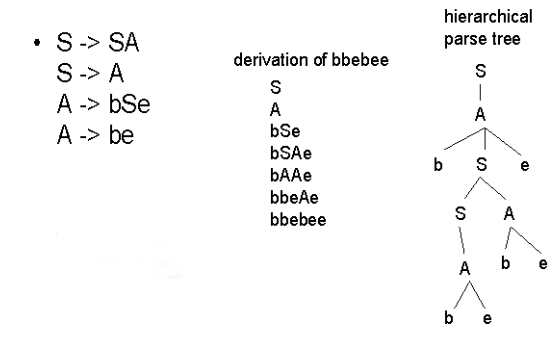
\includegraphics[width=0.7\textwidth]{img/GIC2.png}
    \caption{CFG example \protect\footnote{http://www.biiet.org/blog/wp-content/uploads/2013/07/img028.jpg}}
    \label{fig:CFG}
\end{figure}

%\footnote{http://www.biiet.org/blog/wp-content/uploads/2013/07/img028.jpg}
%falar dos terminais, nao terminais, start symbols e de Noam Chomsky

One valid sentences (Example in Figure ~\ref{fig:CFG}), could be : bbebee .

In the compilers area two major classes of grammars are used : CFG (Context-free grammar) and AG ( Attribute Grammar).

The difference between these two grammars are that a CFG is directed to define the syntax (only) and, AG contains semantic and syntax rules.

An AG is , basically, a GFC grammar extended with semantic definitions. It is a formal way to define attributes for the symbols that occur in each production of the underlying grammar. We can associate values to these attributes later, after processed with a parser; the evaluation will occur applying those semantic definition to any node of the abstract syntax tree.
These attributes are divided into two groups: synthesized attributes and inherited attributes.

The synthesized attributes are the result of the attribute evaluation rules for the root symbol of each subtree, and may also use the values of the inherited attributes. The inherited attributes are passed down from parent nodes to children or between siblings.

Like that it is possible to transport information anywhere in the abstract syntax tree which is one of the strength for using an AG (as seen on Listing ~\ref{lst:ag}).

%put an AG example !

\begin{comment}
\begin{figure}[h!]
  \centering
    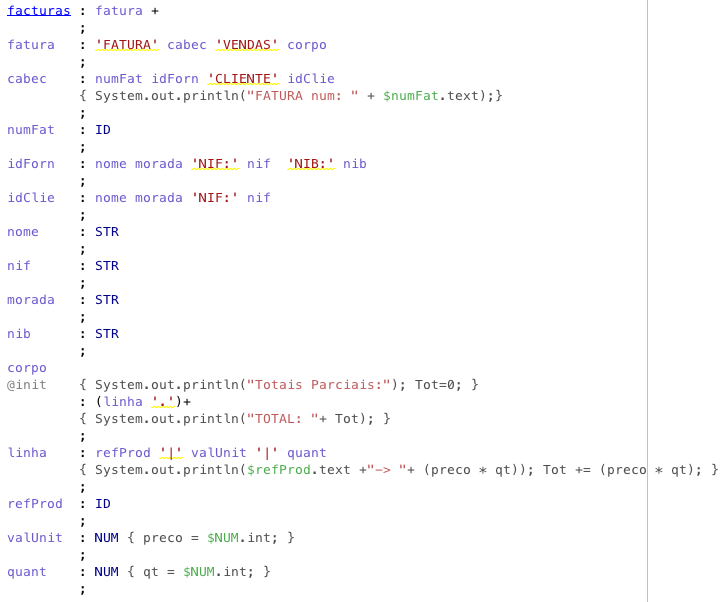
\includegraphics[width=0.9\textwidth]{img/ga.png}
    \caption{Example of an AG}
    \label{fig:GA}
\end{figure}
\end{comment}	

\begin{lstlisting}[caption={Example of an AG},label={lst:ag}]
facturas : fatura (facturas)*
         ;

fatura : 'FATURA' cabec 'VENDAS' corpo {System.out.println("Total Factura: "+$corpo.totOut);}
       ;

cabec : idFat idForn 'CLIENTE' idClie {System.out.println("Factura n: "+$idFat.text);}
      ;

idFat : numFat ;

numFat : ID ;

idForn : nome morada 'NIF:' nif 'NIB:' nib
       ;

idClie : nome morada 'NIF:' nif
       ;

nome :  STR ;

morada : STR;

nif : STR;

nib : STR;

corpo returns [int totOut]
    : linha '.' {$totOut += $linha.linhatot;}
      (linha '.' {$totOut += $linha.linhatot;})*
    ;

linha returns [int linhatot]
      : refProd '|' valUnit '|' quant {$linhatot = $valUnit.val * $quant.quan;System.out.println("Ref: "+$refProd.text+" Total linha: "+($linhatot)+" Euros");}
      ;
	
	refProd : ID;
valUnit returns [int val]
        : NUM {$val = $NUM.int;}
        ;
quant returns [int quan]
    : NUM {$quan = $NUM.int;}
    ;

\end{lstlisting}


In this way, an AG will be used to specify the translation from syntax tree directly into code for some specific machine or into another intermediate language.
For our thesis, the AG will be processed by ANTLR tool in order to build automatically the parser, the attribute evaluator, and the code generation.
%%%%%%%%%%%%%%%%%%%%%%%%%%%%%%%%%%%%%%%%%%%%%%%%%%%%%%

\section{Formal Grammar}
According to Noam Chomsky, a classic formalization of generative grammars is composed by:
\begin{itemize}
        \item A finite set N of nonterminals symbols.
        \item A finite set $\sum$  of terminals symbols.
        \item A finite set P of production rules.
        \item A start symbol S $\in$  P
\end{itemize}
A grammar is formally constructed by that tuple (N,$\sum$,P,S).



Grammar is a set of productions rules which describes the syntax of the language (not semantic). Each grammar has only one start symbol production that defines where the grammar begins.
%And there is two types after that the production rules are then applied in any order.
And each production is composed by two things : LHS (Left Hand Side) and RHS (Right and Side). Left Hand Side represents the non terminal and the right hand side represents the behavior of the rule ( composed by non terminal and terminal).

\begin{lstlisting}[caption={A rule production},label={lst:ruleExample}]
     liss : 'program' identifier body
          ;
\end{lstlisting}

In ~\ref{lst:ruleExample}, we can see that it is composed by two sides. The left hand side and the right hand side, delimited by ':'.
On the LHS, 'liss' is a non-terminal and on the RHS, it is composed by the terminal 'program' followed by two non-terminals.
This is the syntax of one production rule of the grammar.

Now let's speak about the entire syntax of the LISS.

%\subsection{LISS Syntax}
\chapter{LISS language}

LISS ~\citep{CH07a} -that stands for Language of Integers, Sequences and Sets- is an imperative programming language, defined by the Language Processing members (Pedro Henriques and Leonor Barroca) at UM for teaching purposes (compiler course).

The idea behind the design of LISS language was to create a simplified version of the more usual imperative languages although combining functionalities from various languages.

It is designed to have atomic or structured integer values, as well as, control statements and block structure statements.

Now, let's explain the basic statements of the language and its data types as BNF grammar on the next section.

\section{LISS Data types}

There are 5 types available.
From atomic to structured types, they are known as : integer, boolean, array, set and sequence.

Used for declaring a variable on the program, this gives us vital information for understanding what kind of type we are dealing it regarding a certain variable.
Let's see deeper with one LISS code example:

\begin{lstlisting}[caption={Declaring a variable in LISS},label={lst:declare_variable}]
  a -> integer;
  b -> boolean;
  c -> array size 5,4;
  d -> set;
  e -> sequence;
\end{lstlisting}

As we can see in Listing ~\ref{lst:declare_variable}, some variables ('a','b','c','d' and 'e')  are being declared with his own types ('integer', 'boolean', 'array', 'set' and 'sequence').
Synthetically, in LISS, this is done by writing the variable name followed by an arrow and the type of the variable (see Listing ~\ref{lst:variable_declaration_BNF}).

\begin{lstlisting}[caption={BNF of declaring a variable in LISS},label={lst:variable_declaration_BNF}]
variable_declaration : vars '->' type ';'
                     ;
vars : var (',' var )*
     ;
var : identifier value_var
    ;
value_var :
          | '=' inic_var
          ;
type : 'integer'
     | 'boolean'
     | 'set'
     | 'sequence'
     | 'array' 'size' dimension
     ;
dimension : number (',' number )*
          ;
inic_var : constant
         | array_definition
         | set_definition
         | sequence_definition
         ;
constant : sign number
         | 'true'
         | 'false'
         ;
sign :
     | '+'
     | '-'
     ;

\end{lstlisting}

Variables that are not initialized, have a default value (according to Table ~\ref{tbl:data_types}).

\begin{table}[]
\centering
\caption{LISS data types}
\label{tbl:data_types}
\begin{tabular}{|c|c|}
\hline
\textbf{Type}       & \multicolumn{1}{l|}{\textbf{Default Value}} \\ \hline
boolean             & false                                       \\ \hline
integer             & 0                                           \\ \hline
array               & {[}0,...,0{]}                               \\ \hline
set                 & \{\}                                        \\ \hline
sequence            & nil                                         \\ \hline
\end{tabular}
\end{table}

\newpage
Additionally, we may change the values of the variables by initializing them with a different value (see Listing ~\ref{lst:variable_declaration}).
This can be made by putting an equal symbol after the variable name and, then, inserting the right value according to the type (see example in Listing ~\ref{lst:variable_declaration_BNF}).

\begin{lstlisting}[caption={Initialize a variable},label={lst:variable_declaration}]
  a = 4, b -> integer;
  t = true -> boolean;
  vector1 = [1,2,3], vector2 -> array size 5;
  a = { x | x<10} -> set ;
  seq1 = <<10,20,30,40,50>>, seq3 = <<1,2>>, seq2 -> sequence;
\end{lstlisting}

Now, let's see and list which type are, correctly, associated with the arithmetic symbols and functions in LISS (see Table ~\ref{tbl:type_operations}).


\begin{table}[]
\centering
\caption{Operations and signatures in LISS}
\label{tbl:type_operations}
\begin{tabular}{|c|c|}
\hline
\textbf{Symbols \&\& Functions} & \multicolumn{1}{l|}{\textbf{Signatures}} \\ \hline
+ (add)                                   & integer x integer \verb+->+ integer                                        \\ \hline
- (subtract)                              & integer x integer \verb+->+ integer                                        \\ \hline
\verb+||+ (or)                            & boolean x boolean  \verb+->+ boolean                                       \\ \hline
++ (union)                                & set x set \verb+->+ set                                                    \\ \hline
/ (division)                              & integer x integer \verb+->+ integer                                        \\ \hline
* (multiply)                              & integer x integer \verb+->+ integer                                        \\ \hline
\&\& (and)                                & boolean x boolean \verb+->+ boolean                                        \\ \hline
** (intersection)                         & set x set \verb+->+ set                                                    \\ \hline
== (equal)                                & integer x integer \verb+->+ integer; boolean x boolean \verb+->+ boolean   \\ \hline
!= (not equal)                            & integer x integer \verb+->+ integer; boolean x boolean \verb+->+ boolean   \\ \hline
\textless  (less than)                    & integer x integer \verb+->+ integer                                        \\ \hline
\textgreater  (greater than)              & integer x integer \verb+->+ integer                                        \\ \hline
\textless= (less than or equal to)        & integer x integer \verb+->+ integer                                        \\ \hline
\textgreater= (great than or equal to)    & integer x integer \verb+->+ integer                                        \\ \hline
in (contains)                              & integer x set \verb+->+ boolean                                            \\ \hline
tail                                      & sequence \verb+->+ sequence                                                \\ \hline
head                                      & sequence \verb+->+ integer                                                 \\ \hline
cons                                      & integer x sequence \verb+->+ sequence                                      \\ \hline
delete                                    & integer x sequence \verb+->+ sequence                                      \\ \hline
copy                                      & sequence x sequence \verb+->+ void                                         \\ \hline
cat                                       & sequence x sequence \verb+->+ void                                         \\ \hline
isEmpty                                   & sequence \verb+->+ boolean                                                 \\ \hline
length                                    & sequence \verb+->+ integer                                                 \\ \hline
isMember                                  & integer x sequence \verb+->+ boolean                                       \\ \hline
\end{tabular}
\end{table}

\newpage

So, in Table ~\ref{tbl:type_operations}, we list the symbols and functions, who are available in LISS, and also its signature associated.
In order to understand the table better, we will explain how to read the symbol and its signature with one example.

For example, the symbol '+' indicates that it can operate with, only, integers on each side of the symbol (separated by the symbol 'x') and that, the result of that operation, indicated by the symbol '\verb+->+', will be an integer.
%Notice that semantically, operations must be validated according to the table ~\ref{tbl:type_operations}, otherwise the operations would be incorrect and throw an error.
Semantically, operations must be validated according to table ~\ref{tbl:type_operations}, otherwise the operations would be incorrect and throw an error.

\bigbreak

\textbf{Arrays.}
LISS supports a way in indexing a collections of integer values such that each value is uniquely addressed (also it supports one great and most important property of being multidimensional).

Called as 'array', it is considered to be a static structured type due to the fact that his dimension and maximum size of elements is fixed at the declaration time.

%One of its, most important, property is that he may have multiple dimension.

And the operations defined over an array are basic in LISS:

\begin{enumerate}
\item \textit{indexing} %- denoted by '[' and ']', it selects the value of the chosen indexed array.
\item \textit{assignment} %- 
\end{enumerate}

%explaining probably indexing and assignment

Arrays can be initialized, in the declaration section, partially or completely the elements of each dimension.
For example, consider an array of dimension 3x2 with the following way:

\begin{lstlisting}
  array1 = [[1,2],[5]] -> array size 3,2;
\end{lstlisting} 

Thi is equivalent to the initialization below:

\begin{lstlisting}
  array1 = [[1,2],[5,0],[0,0]] -> array size 3,2;
\end{lstlisting}

Notice that the elements who weren't declared, are initialized with the value 0 (see Table ~\ref{tbl:data_types}).

The grammar who rules behind the syntax for array declaration and initialization is shown below.

\begin{lstlisting}
  array_definition : '[' array_initialization ']'
                 ;

  array_initialization : elem (',' elem)*
                     ;

  elem : number
     | array_definition
     ;
\end{lstlisting}

\bigbreak

\textbf{Sets.}
The type \textit{set} in LISS, is a collection of integers with no repeated numbers.
It operates with a comprehension list instead of an enumeration.
Set type can operates with two different ways.
The first one is the empty value and this means that the set is empty. Syntactically, this is done by writing '\verb+{}+'.

The other one is an 'identifier' separated by an explicit symbol '\verb+|+' and an 'expression'. Expression is a set of operations that, at the end, result must be a boolean. Otherwise the set won't work

The operations defined for sets are :
\begin{enumerate}
\item \textit{union}
\item \textit{intersection}
\item \textit{in}
\end{enumerate}


Let's see an example of its syntax below:

\begin{lstlisting}
  set1 = {x | x < 6 && x > -7} -> set;
\end{lstlisting}

This set explain us that only integers from -7 to 6 are valid and every others numbers are not included on the set.

The syntax for set declaration and initialization is :

\begin{lstlisting}
  set_definition : '{' set_initialization '}'
               ;

  set_initialization :
                   | identifier '|' expression
                   ;
\end{lstlisting}

\bigbreak

\textbf{Sequences.}
Considered as an array of one dimension, the type sequence is a collection of a list ordered integers. But, instead of the concept of an array, its size is not fixed; this means that it grows dinamicallly at run time like a linked list.
There is two ways in defining sequences.
The first way is declaring it with the empty value (syntactically done by writing '\verb+<<>>+') and the second way is by defining with integers to the sequence.
Let's see deeper with one example:

\begin{lstlisting}[caption={Example of valid operations using sequence on LISS},label={lst:sequence_example_use}]
  c=<<1,2,3>> -> sequence;
\end{lstlisting}

So, the sequence example is defined by three numbers (3,2,1). 
Also some operations are defined for the sequence type and they are known as:
\begin{enumerate}
\item \textit{tail}
\item \textit{head}
\item \textit{cons}
\item \textit{delete}
\item \textit{copy}
\item \textit{cat}
\item \textit{isEmpty}
\item \textit{length}
\item \textit{isMember}
\end{enumerate}
Those operations will be explained further and deeper.

Now, the grammar behind the type sequence is defined by the follow one:

\begin{lstlisting}
  sequence_definition : '<<' sequence_initialization '>>'
                    ;

  sequence_initialization :
                        | values
                        ;

  values : number (',' number )*
       ;

\end{lstlisting}





%%%%%%%%%%%%%%%%%%%%%%%%%%%%%%%%%%%%%%%%%%%%%%%%%%%%%%%%%%%%%%%%%%%%%%%%%%%%%%%%%%%%%%%%%%%%%%%%%%%%%%%%%%%%%%%%%%%%%%%%%%%%%%%%%%%%%%%%%%%%%%%%%%%%%%%%%%%

\begin{comment}

However, there are restrictions on the syntactic and semantic levels on those types which we must list them below.
Integer type operates with integer values, thus we can add or not, a sign to the integer value (see in Listing ~\ref{lst:integer_example_use}.

\begin{lstlisting}[caption={Example of valid operations using integers on LISS},label={lst:integer_example_use}]
a, b=2, c=+2, d=-3 -> integer;
\end{lstlisting}

Boolean type operates with only boolean values (see in Listing ~\ref{lst:boolean_example_use}).

\begin{lstlisting}[caption={Example of valid operations using booleans on LISS},label={lst:boolean_example_use}]
a, b=true, c=false -> boolean;
\end{lstlisting}

Set type can operates with two different ways.
The first one is the empty value and this means that the set is empty. Syntactically, this is done by writing '{}'.

The other one is an identifier separated by an explicit symbol '|' and an expression. Expression is a set of operations that, at the end, result must be a boolean. Otherwise the set won't work (see in Listing ~\ref{lst:}). 

\begin{lstlisting}[caption={Example of valid operations using set on LISS},label={lst:set_example_use}]
a, b={}, c={e|e+1==10} -> set;
\end{lstlisting}

Sequence type also have the same system of set type. 
This means that it has the option to have an empty value or add values to the sequence.
The empty value is, syntactically, done by writing '<<>>'. On the other hand, we can add only integers to the sequence, if the sequence is not empty (see in Listing ~\ref{lst:sequence_example_use}).

\begin{lstlisting}[caption={Example of valid operations using sequence on LISS},label={lst:sequence_example_use}]
a, b=<<>>, c=<<1,2,3>> -> sequence;
\end{lstlisting}

\end{comment}
%%%%%%%%%%%%%%%%%%%%%%%%%%%%%%%%%%%%%%%%%%%%%%%%%%%%%%%%%%%%%%%%%%%%%%%%%%%%%%%%%%%%%%%%%%%%%%%%%%%%%%%%%%%%%%%%%%%%%%%%%%%%%%%%%%%%%%%%%%%%%%%%%%%%%%%%%%%

%\section{Blocks and Control statements}
\section{LISS blocks and statements}

A LISS program is always composed of two parts: declarations and statements (a program block).
LISS language is structured with ease and simple hierarchy.
And this is done by structuring LISS code as a block.

It begins by creating our program with a name, succeeding by implementing the declaration of variables and then the flow of the program by writing statements.
Let's see a deeper look with one example (see Listing ~\ref{lst:block_liss}).

\begin{lstlisting}[caption={The structure of a LISS program (example)},label={lst:block_liss}]
program sum{
    declarations
        int=2 -> integer;
    statements
        writeln(int+3);
}
\end{lstlisting}

So a program in LISS, begins by, syntactically, writing 'program' and then the name of the program (in this case, the name is 'sum').
Then appears some braces that delimits the contents of the program which is done by opening it after the name of the program and closing it at the end of the program.
After those braces, there is one important part to alert the user with the way of declaring variables and statements.

As in a traditional imperative language (let's compare 'C language'), if we don't take the habits of implementing the variable always in a certain part of the code. We may be confused by implementing and finding them randomly in the code. And this makes the life harder to the programmer in understanding the code when the code is quite long/bigger.

So, in LISS, we always declare variable declarations firstly (syntactically written by 'declarations')  and then the statements secondly (syntactically written by 'statements').
This is due to the fact that LISS want to help the user by creating solid and correctness code. And in this case, the user will always know that all the variable declarations will be always at the top of the statements and not randomly everywhere. 

Then, comes the part where we implement the flow of the program under the section of 'statements'.

\subsection{Statements}

As said previously, under the statements part, we control and implement the flow of LISS program.
In LISS, we may write none or multiple statements consecutively and notice that the same behavior is, also, done for declaring variables.

Every statements ends with a semicolon unless two type of statements (conditional and cyclic/iterative statement) (as shown in Listing ~\ref{lst:liss_statements_bnf}).
%One important thing to mention is the fact that almost every statements ends with a semicolon unless conditional or cyclic/iterative statements.

\begin{lstlisting}[caption={BNF of statements in LISS},label={lst:liss_statements_bnf}]
statements : statement*
           ;
statement : assignment ';'
          | write_statement ';'
          | read_statement ';'
          | conditional_statement
          | iterative_statement
          | function_call ';'
          | succ_or_pred ';'
          | copy_statement ';'
          | cat_statement ';'
          ;
\end{lstlisting}

Let's see one example of a LISS program which shows how it is done (see in Listing ~\ref{lst:statements_example}).

\begin{lstlisting}[caption={Example of using statements in LISS},label={lst:statements_example}]
program factorial{
    declarations
        res=1, i=5 -> integer;
    statements
        writeln(res);
        for(j in 1..i){
            res=res*j;
        }
        writeln(res);
}
\end{lstlisting}




\subsection{Control statements}

LISS language includes some statements for controlling the execution flow at runtime with two different kind of behavior.

The first one is called conditional statement and it has only one variant in LISS language (see Listing ~\ref{lst:control_statements}).

But the second one is called cyclic statement or iterative statement, and it has two cyclic different variants (see Listing ~\ref{lst:control_statements}).

\begin{lstlisting}[caption={BNF of control statements in LISS},label={lst:control_statements}]
conditional_statement : if_then_else_stat
                      ;
iterative_statement : for_stat
                    | while_stat
                    ;
\end{lstlisting}

These control statements, mimics the syntax and the behavior, nearly,  of other modern imperative language.
But, we should take a look on the behavior of one of the control statement in order to understand its role deeper.

The 'for' statement has two different ways for defining his comportment.
Normally, in a conventional way, the for-loop has a control variable which takes a value in a given range and step up or step down by a default or a explicit value.

In LISS, the control variable is set in a given integer interval defined by the lower and upper bounds. Therefore, by default, the step is incremented by one but it is possible to increment or decrease it by setting it explicitly.
Additionally, we may write a condition for filtering on each step the for-loop statement, like setting an if-condition.
This can be done with the following syntax:
\begin{lstlisting}[caption={LISS syntax of a for-loop statement},label={lst:for-loop}]
for(a in 1..10) stepUp 2 satisfying array[a]==1{
	...
}
\end{lstlisting}
In Listing ~\ref{lst:for-loop}, the control variable 'a' is set to a range by 1 to 10 and would be increased (due to 'stepUp' syntax) by 2. Also there is a filter condition which is applied after the 'satisfying' syntax and it will be tested on each step of the for-loop statement. Notice that the filter condition must boolean and that if it pass the condition, then the inner content of the for-loop statement would be executed. 

Otherwise the control variable would be incremented with the explicit value 2 and the filter condition tested again. 
This is the first example, about expressing in a way the for-loop statement. Let's see the second way on the next lines.

There is also the possibility for ease use, in expressing a for-each statement on a array.
And this is done by calling a simple syntax in LISS.

\begin{lstlisting}[caption={LISS syntax of a for-each statement on array},label={lst:for-each_array}]
for(b inArray array){
	...
}
\end{lstlisting}
In Listing ~\ref{lst:for-each_array}, the control variable  'b' is assigned with all of the elements of the array and begins with his lower index (zero) until his upper index (size of the array minus one).
Notice that, in this case, we cannot apply an increment or decrement behavior and also a filter condition.

The next grammar fragment describes the cycle for in LISS:

\begin{lstlisting}[caption={BNF of for statement in LISS}]
for_stat : 'for' '(' interval ')' step satisfy
           '{' statements '}'
         ;
interval : identifier type_interval
         ;
type_interval : 'in' range
              | 'inArray' identifier
              ;
range : minimum '..' maximum
      ;
minimum : number
        | identifier
        ;
maximum : number
        | identifier
        ;
step :
     | up_down number
     ;
up_down : 'stepUp'
        | 'stepDown'
        ;
satisfy :
        | 'satisfying' expression
        ;
\end{lstlisting}

%write the for statetement with step and satisfy explication


\section{Subprograms}

In LISS, it is possible to organize your code by splitting a portion of your code into sub-programs. This allows to the programmer to reuse or give more clarity to his code by creating functions or doing some procedure.
Also, it is possible to create sub-programs into sub-programs by using a nesting strategy.

The syntax who defines a sub-program in LISS is shown in Listing ~\ref{lst:block_structure}.

\begin{lstlisting}[caption={BNF of block structure in LISS},label={lst:block_structure}]
subprogram_definition: 'subprogram' identifier '(' formal_args ')' return_type f_body
                     ;
f_body : '{'
         'declarations' declarations
         'statements' statements
         returnSubPrg
         '}'
       ;
formal_args :
            | f_args
            ;
f_args  : formal_arg (',' formal_arg )*
        ;
formal_arg : identifier '->' type
           ;
return_type :
            | '->' typeReturnSubProgram
            ;
returnSubPrg :
             | 'return' expression ';'
             ;
\end{lstlisting}

Note that every variable, who are declared inside of a sub-program, are local, and they can be access to others nested sub-program of a sub-program.
However, variables declared in the program (not in a sub-program) are considered global and not local.










%Also, in LISS language, variables are declared firstly and then we may code the program.
%Notice that this restriction is done for a better experience of the programmer. 
%This means that variables must be declared always on top of the program before they will be used on the rest of the program.


%It allows handling integers, sets of integers, dynamic sequences, complex numbers, polynomials, etc., etc~\citep{CH07d,CH07a,CH06a,CH06b,CH05a}.


\newpage


%write appendix , code gic liss

\section{Evolution of LISS syntax}
Due to the maturity of the language already done by the professors whom invented, we have added some few but extra changes for a better experience of the programming language.
The syntax of the LISS language (Figure ~\ref{lst:GIC_LISS} ), has been constructed with ANTLR which is ANother Tool for Language Recognition where it collaborates with the Java platform.

One of the first objectives is that we have changed the format of the syntax. We have translated the old LISS language to a brand new extended BNF format (as shown in Figure ~\ref{lst:GIC_LISS}).

Then we have added some better clarification syntactically of the programming language which was by not mixing functions and variable declarations between them (See Figure ~\ref{lst:declaration_LISS}).
Like that we, indirectly, teach the programmer by doing it in the right way. So we declare, firstly, the variables and then the functions.
\begin{lstlisting}[caption={},label={lst:declaration_LISS}]
declaration : variable_declaration * subprogram_definition *
            ;
\end{lstlisting}

Another objectives was to add punctuation after each line of any statements (See Figure ~\ref{lst:statement_LISS}).
\begin{lstlisting}[caption={Function statement},label={lst:statement_LISS}]
statement : assignment  ';'
          | write_statement  ';'
          | read_statement  ';'
          | conditional_statement
          | iterative_statement
          | function_call ';'
          | succ_or_pred  ';'
          | copy_statement  ';'
          | cat_statement  ';'
          ;
\end{lstlisting}

As adding also a 'cat\_statement' rule which works with only sets. It concatenate sets with another sets.

Regarding to the arrays, it was previously able to add some expressions over the access elements of the array. But these access were able to use some boolean expression which was non sense regarding to the semantic. So we changed and allowed any other expressions less than boolean expression (See figure ~\ref{lst:elem_array_LISS}).


\begin{lstlisting}[caption={Rule element of array},label={lst:elem_array_LISS}]
elem_array : single_expression (',' s2=single_expression )*
           ;
\end{lstlisting}

In the previous version of the LISS, it was allowed to create a big boolean expression, but we decided to change that and only able to create one boolean expression (See figure ~\ref{lst:expression_LISS}).
It was a non sense of having an expression like that : '3 == 4 == 5 != 6'.
\begin{lstlisting}[caption={Rule expression},label={lst:expression_LISS}]
expression : single_expression (rel_op single_expression )?
           ;
\end{lstlisting}

We added the possibility of using some parenthesis over expressions (See figure ~\ref{lst:factor_LISS}).

\begin{lstlisting}[caption={Rule factor},label={lst:factor_LISS}]
factor: '(' expression ')'
      ;
\end{lstlisting}

We changed the rules of two functions: 'cons' and 'del'. These functions were working with both in the same way. Waiting for an expression and a variable as arguments. Now, we decided to change that and giving more powers of expressivity to those functions ~\ref{lst:cons_del_LISS}.

\begin{lstlisting}[caption={Rule cons and delete},label={lst:cons_del_LISS}]
cons // integer x sequence -> sequence
     : 'cons' '(' expression ',' expression ')'
     ;

delete // del : integer x sequence -> sequence
       : 'del' '(' expression ',' expression ')'
       ;
\end{lstlisting}

Beside of adding some improvements to the grammar, we additionally deleted a rule which we thought it wasn't necessary to have (see figure ~\ref{lst:type_interval_LISS}).
\begin{lstlisting}[caption={Rule type interval},label={lst:type_interval_LISS}]
type_interval : 'in' range
              | 'inArray' identifier
              //| 'inFunction' identifier
              ;
\end{lstlisting}

Last but not least, we also added the way of adding some comments to the programming language. Giving more power for the user in giving some informations about his code.

\begin{lstlisting}[caption={Rule comment},label={lst:comments_LISS}]
fragment
COMMENT
    : '/*'.*?'*/' /* multiple comments*/
    | '//'~('\r' | '\n')* /* single comment*/
    ;
\end{lstlisting}


%\section{MIPS}
\chapter{Target machine}

%As mentioned in the previous section, the AG will produce MIPS assembly code throw ANTLR.

\section{MIPS}
MIPS, from Microprocessor without Interlocked Pipeline Stages, is a reduced instruction set computer (RISC) developed by MIPS Technologies. % creating low-level programming language.
%It is a symbolic representation of machine instructions.


%composto o cpu, descodificador, o controlador, RAM, os registos e alem disto os 5 tipo de instruçoes
The architecture of MIPS is composed by 5 stages (see Figure ~\ref{fig:MIPSarchitecture}).

\begin{figure}[h!]
  \centering
    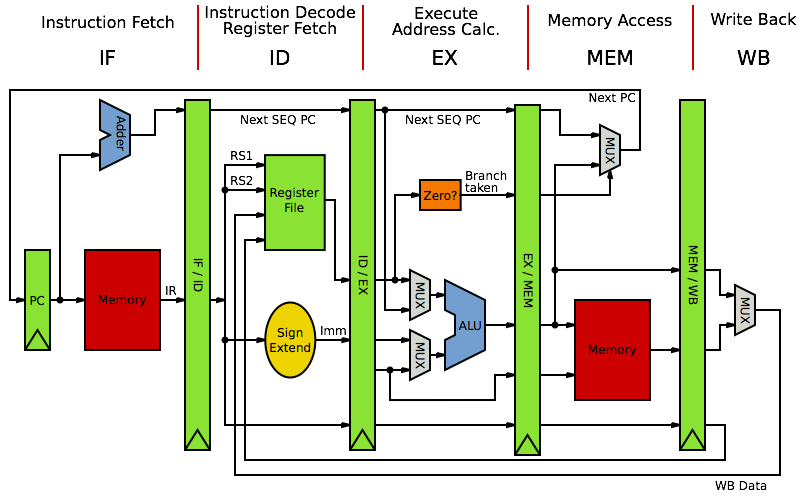
\includegraphics[width=1\textwidth]{img/MIPSarchitecture.png}
    \caption{MIPS architecture \protect\footnote{http://upload.wikimedia.org/wikipedia/commons/thumb/e/ea/MIPS\_Architecture(Pipelined).svg/300px-MIPS\_Architecture\_(Pipelined).svg.png}}
    \label{fig:MIPSarchitecture}
\end{figure}

%\protect\footnote{http://upload.wikimedia.org/wikipedia/commons/thumb/e/ea/MIPS_Architecture_(Pipelined).svg/300px-MIPS_Architecture_(Pipelined).svg.png}

\newpage

It has 32 registers and 5 type of instructions :

\begin{itemize}
  \item instructions for data transfer
  \item instructions for arithmetic
  \item instructions for logical
  \item instructions for conditional branch
  \item instructions for unconditional jump

\end{itemize}

 %( instructions for data transfer, arithmetic, logical, conditional branch, unconditional jump).

It uses a mnemonic to represent each low-level machine instruction or operation.
Operations require three operands in order to form a complete instruction in MIPS assembly code, the address for the result and the address of the two operands.

A simple example of a complete instruction can be seen in Listing ~\ref{lst:addMIPS}.

\begin{lstlisting}[caption={Sum of two registers in MIPS assembly code},label={lst:addMIPS}]
  add  $s1,$s2,$s3
\end{lstlisting}

The instruction shown in Listing ~\ref{lst:addMIPS}, means that register \$s2 shall be added to register \$s3 and their sum (the result) stored in \$s1 register (note that each operand is represented by \$ sign).

As mentioned in the previous section, the AG processed by the compiler generator ANTLR will compose MIPS assembly. The MIPS assembly instructions generated so far will be converted into executable machine code by an assembler included in MARS environment (a MIPS simulator and debugger) according to the process depicted in Figure ~\ref{fig:hl2ll}.


\begin{figure}[h!]
  \centering
    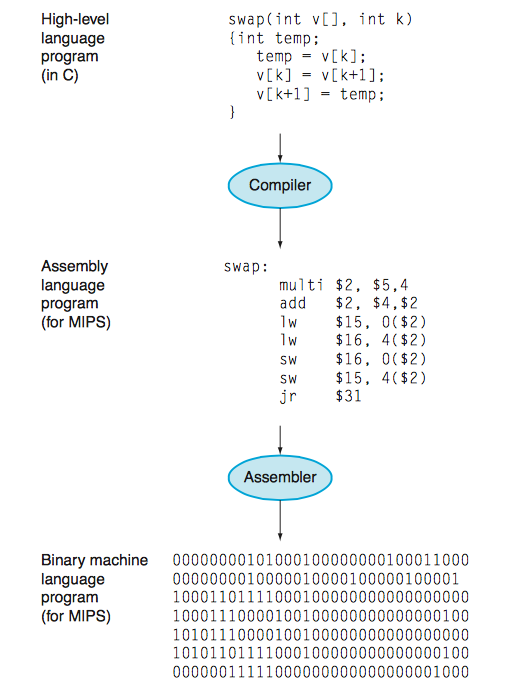
\includegraphics[height=0.9\textwidth]{img/high-level-2-low-level.png}
    \caption{Stages converting high-level language into binary machine language \protect\footnote{\cite{DAPJLH}}}
    \label{fig:hl2ll}
\end{figure}



%\section{Citations}
%Example of a citation: \cite{GRM97}, cf.\ this entry in the \Bibtex\ file.
%Another way of citing is \citep{KeR88}

%\section{Optional}
%You may wish to use the \conexp{Concept-Explorer} tool.

%\chapter{The problem and its challenges}


After presenting in the previous chapter the essential definitions for the intended work, in this chapter the project planned for this master thesis will be explained.

%Firstly, there is the necessity of generating the GIC from LISS language, like that we will see if there is no problem with the rules and definitions of a well grammar and follow the same grammar as LISS language (not being distinct) using ANTLR tool.

First, create an ANTLR version of the CFG grammar for LISS language.


Second, extend the LISS CFG to an AG in order to specify throw it the generation of MIPS assembly code.
To verify the correctness of the assembly code generated, a simple MIPS simulator, named MARS, will be selected to provide all the tools for checking it.

Third, the desired Structure-Editor, SDE, will be developed based on ANTLR.
It will be implemented in with Java SWING because ANTLR has always been implemented via Java and it is said, also, to use Java target as a reference implementation mirrored by other targets.
SWING is a GUI widget toolkit for Java which provides all the API for creating an interface with Java.
At this phase, we will create an IDE similar to other platforms but with the capacity of being a syntax-directed editor.

Fourthly, to complete the SDE functionality, an incremental compiler shall be included.
Incremental compilation ~\citep{RTD83a,Hol87a,VSK90a} means that only the part that was changed must be processed again. And like that, both tasks (edition and compilation) are done synchronously at the same time and having an editor which compiles cleverly.

Finally, exhaustive and relevant tests will be made with the tool created and, the outcomes will be analyzed and discussed.

%\section*{LISS language}


%\section{Assembly code MIPS}

%que se deve falar ?

%         The problem and its challenges.

%\section{Images}
%       Example of inserting an image as displyed text,
%\begin{center}
%       
\includegraphics[width=0.2\textwidth]{img/mei-logo-03.jpg}
%\end{center}

%\begin{wrapfigure}{r}{0.25\textwidth}
%       
\includegraphics[width=0.2\textwidth]{img/mei-logo-03.jpg}
%\end{wrapfigure}
%\noindent --- wrapped into the text,
%bla-bla bla-bla bla-bla bla-bla bla-bla bla-bla bla-bla bla-bla bla-bla bla-bla
%bla-bla bla-bla bla-bla bla-bla bla-bla bla-bla bla-bla bla-bla bla-bla bla-bla
%bla-bla bla-bla bla-bla bla-bla bla-bla bla-bla bla-bla bla-bla bla-bla bla-bla
%bla-bla bla-bla bla-bla bla-bla bla-bla bla-bla bla-bla bla-bla bla-bla bla-bla
%bla-bla bla-bla bla-bla bla-bla bla-bla bla-bla bla-bla bla-bla bla-bla bla-bla bla-bla bla-bla bla-bla bla-bla
%bla-bla bla-bla bla-bla bla-bla bla-bla bla-bla bla-bla bla-bla bla-bla bla-bla bla-bla bla-bla bla-bla bla-bla

%\noindent --- or as a floating body.
%\begin{figure}
%\begin{center}
%       
\includegraphics[width=0.5\textwidth]{img/mei-logo-03.jpg}
%\end{center}
%\caption{caption}
%\end{figure}

%You can also use an image as an icon, eg.\ \MEI, in the main tex.
%Click on it to visit the website. It is also listed in the list of terms.
%Another example of an item to appear in the term index: \UM (needs \Makeindex)


%\part{Core of the dissertation}

%\part{Core of the dissertation}

\chapter{Compiler development}
%       Main result(s) and their scientific evidence
%\section{Introduction}
Earlier in the history of computers, software was primarily written in assembly language. Due to the low productivity of programming assembly code, researchers invented a way that add some more productivity and flexibility for programmers; they created the compiler allowing to wire programs in high level programming languages.

A compiler is a software program which converts a high-level programming language (source code) into a lower level programing language for the target machine (known as machine code or assembly language).

The compiler task is divided into several steps (see Figure \ref{fig:compiler}):
\begin{enumerate}
  \item Lexical analysis
  \item Syntactic analysis or parsing
  \item Semantic analysis
  \item Optimization
  \item Code generation
\end{enumerate}

\begin{figure}
\begin{center}
       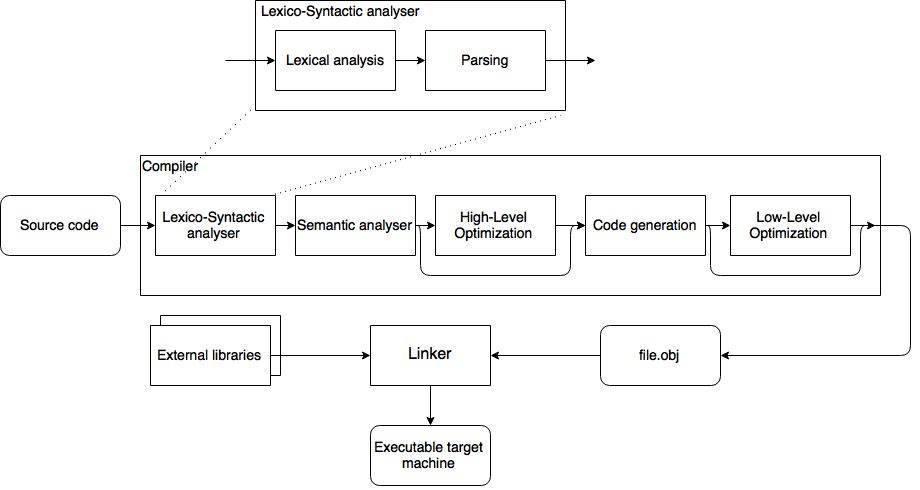
\includegraphics[width=1\textwidth]{img/compiler.png}
\end{center}
\caption{Traditional compiler}
\label{fig:compiler}
\end{figure}
\newpage
The task of constructing a compiler for a particular source language is complex. Firstly, the lexical analysis must recognize words; these words are a string of symbols each of which is a letter, a digit or a special character.

The Lexical analysis divides program text into "words" or "tokens" and once words are identified, the next step is to understand sentence structure (role of the parser).
We can think the parsing as an analogy of our world by constructing phrases which requires a subject, verb and object. So, basically, the parser do a diagramming of sentences (see Figure \ref{fig:parsing}).
\begin{figure}
\begin{center}
       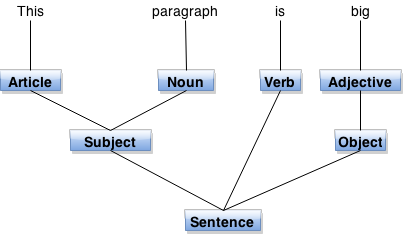
\includegraphics[width=0.7\textwidth]{img/parsing.png}
\end{center}
\caption{Parsing}
\label{fig:parsing}
\end{figure}
%\newpage
Once the sentence structure is understood, we must extract the "meaning" with the semantic analyzer.
The duty of the semantic analyzer is to perform some semantic analysis to catch some inconsistencies.
Finally, after that, it may or may not have some optimization regarding the source code. Then the code generator translates the intermediate representation of the high-level programming into assembly code (lower level programming).
\newpage
%%%%%%%%%%%%%%%%%%%%%%%%%%%

%\section{Summary}
%\section{ANTLR}
\section{Compiler generation with ANTLR}

Terence Parr, the man who is behind ANTLR (ANother Tool for Language Recognition ~\citep{parr2007,Par05}) made a parser (or more precisely, a compiler) generator that reads a context free grammar, a translation grammar, or an attribute grammar and produces automatically a processor (based on a LL(k) recursive-descent parser) for the language defined by the input grammar.

An ANTLR specification is composed by two parts : the one with all the grammar rules and the other one with lexer grammar.

Listing ~\ref{lst:agANTLR} is the one with the grammar rules; in that case it is an  example of an AG.

\begin{comment}
\begin{figure}[h!]
  \centering
    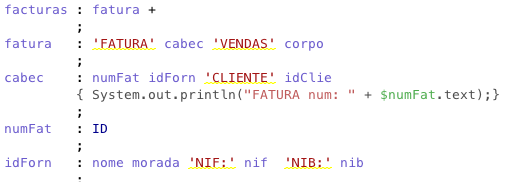
\includegraphics[width=0.8\textwidth]{img/gaAnTLR.png}
    \caption{GA representation on ANTLR}
    \label{fig:gaAntlr}
\end{figure}
\end{comment}

\begin{lstlisting}[caption={AG representation on ANTLR},label={lst:agANTLR}]
facturas : fatura +
         ;
fatura   : 'FATURA' cabec 'VENDAS' corpo
         ;
cabec    : numFat idForn 'CLIENTE' idClie
         { System.out.println("FATURA num: " + $numFat.text);}
         ;
numFat   : ID
         ;
idForn   : nome morada 'NIF:' nif  'NIB:' nib
\end{lstlisting}


On the other hand, the lexer grammar defines the lexical rules which are regular expressions as can be seen in Listing ~\ref{lst:lexer}. They define the set of possible character sequences that are used to form individual tokens. A lexer recognizes strings and for each string found, it produces the respective tokens. %(see figure~\ref{lst:lexer}).

\begin{comment}
\begin{figure}[h!]
  \centering
    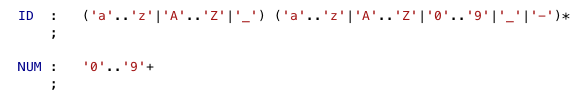
\includegraphics[width=0.8\textwidth]{img/lexer.png}
    \caption{Lexer representation}
    \label{fig:lexer}
\end{figure}
\end{comment}

\begin{lstlisting}[caption={Lexer representation},label={lst:lexer}]
/*--------------- Lexer ---------------------------------------*/

ID  :   ('a'..'z'|'A'..'Z'|'_') ('a'..'z'|'A'..'Z'|'0'..'9'|'_'|'-')*
    ;

NUM :   '0'..'9'+
\end{lstlisting}



%\newpage
The parser generator by ANTLR will be able to create an abstract syntax tree (AST) which is a tree representation of the abstract syntactic structure of source code written in a programming language (see Figure~\ref{fig:AST}).

\begin{figure}[h!]
  \centering
    
\includegraphics[width=1\textwidth]{img/antlr4_parse_tree.png}
    \caption{AST representation}
    \label{fig:AST}
\end{figure}

ANTLR will be used to generate MIPS assembly code according to the semantic rule specified in the AG for LISS language.

%The lexical syntax is usually a regular language, with the grammar rules consisting of regular expressions; they define the set of possible character sequences that are used to form individual tokens or lexemes. A lexer recognizes strings, and for each kind of string found the lexical program takes an action, most simply producing a token.


%\chapter{Applications}
%        Application of main result (examples and case studies)
%\section{Introduction}
%\section{Summary}


%%%%%%%%%%%%%%%%%%%%%%%%%%%%%%%%%%%%%%%%%%%%%%%%%%%%%%%%%%

\chapter{SDE: DEVELOPMENT}

Before we try to explain the concept of a Syntax-Directed Editor (SDE) ~\citep{RT89b,Ko05,alsCH10a,TR81a,RMT86a,RT89a,AHW89}, let's start defining what is an Integrated Development Environment (IDE).

An IDE is described as a software application that provides facilities to computer programmers for software development. It consists , normally, of a source code editor, a compiler, a debugger, and others tools.
IDEs are designed for maximizing the productivity of programmers with visual interface and contains, normally, an interpreter, a compiler or both (see Figure~\ref{fig:ideXCode}).
%IDEs are designed for maximizing the productivity of programmers with visual interface and contains, normally, an interpreter, a compiler or both (see Figure~\ref{fig:ideXCode}).


\begin{figure}[h!]
  \centering
    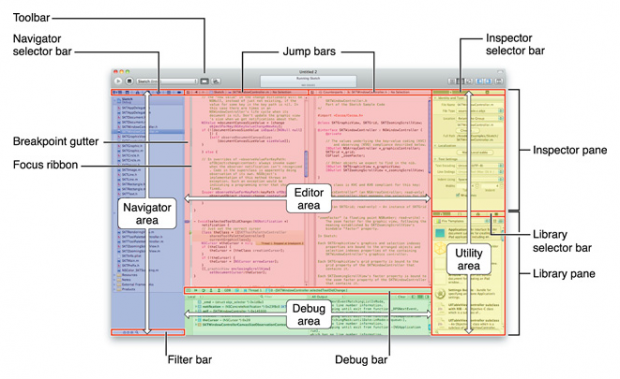
\includegraphics[width=1\textwidth]{img/XCode-interface.png}
    \caption{Example of an IDE visual interface (XCode) \protect\footnote{http://www.alauda.ro/wp-content/uploads/2011/04/XCode-interface-e1302035068112.png}}
    \label{fig:ideXCode}
\end{figure}

\newpage

Programs are created top down in the editor sections by inserting statements and expressions at the right cursor position of the current syntactic template and we can, by the cursor, change simply from one line of text to another one.

A SDE has the same approach of an IDE which is (as said above) an interactive programming environment with integrated facilities to create, edit, execute and debugging programs.
The difference between them is that SDE encourages the program writing at a high level of abstraction, and promotes the programming based on a step by step refinement process.

It liberates the user from knowing the language syntactic details while editing programs.

SDE is basically guided by the syntactic structure of a programming language in both editing and execution. It is a hybrid system between a tree editor and a text editor.

The notion of cursor is really important in the context of SDE because, when the editing mode is on, the cursor is always located in a placeholder of a correct template (see next section) and the programmer may only change to another correct template at that placeholder or to its constituents.%, and not simply from one line of text to another as an IDE alike .
%And the only place where the cursor can move anywhere is in a phrase, which can only be placed at the leftmost symbol of a template or a placeholder.

It reinforces the idea that the program is a hierarchical composition of syntactic objects, rather than a sequence of characters.

\section {What is a template?}

The grammar of a programming language is a collection of production (or derivation rules) that state how a non-terminal symbol (LHS) is decomposed in a sequence of other symbols (RHS). A template is just the RHS of a grammar rule.
Templates cannot be altered, they have placeholders for inserting a phrase or another template and they are generated by editor commands, according to the grammar production. %verificar se pode ou nao inserir placeholders


%meter example of templates !
\begin{lstlisting}[caption={Example of a IF Conditional template},label={lst:template}]
IF( condition )
  THEN statement
  ELSE statement
\end{lstlisting}

In Listing ~\ref{lst:template} we can see the editor template for the if-statement, where \textit{condition} and \textit{statement} are placeholders.

The notion of template is very important because templates are always syntactically correct for two reasons:

\begin{enumerate}
  \item First, the command is validated to guarantee that it inserts a template permitted. %at the current cursor.

  \item Second, the template is not typed, so it contains no lexical errors.

\end{enumerate}

So a correct program (i.e., a valid sentence of the programming language) is created by choosing templates and replacing placeholders by others templates or by concrets values (numeric or string constants or identifiers).

%For a better vision of the context of a SDE, see the figure ~\ref{fig:SDE}.

To clarify the definition of SDE, we will explain it with the help of an example.

\begin{figure}[h!]
  \centering
    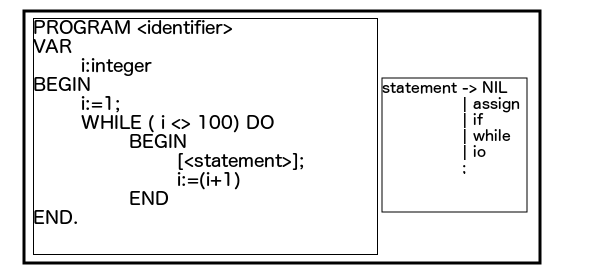
\includegraphics[width=1\textwidth]{img/SDE.png}
    \caption{SDE example}
    \label{fig:SDE}
\end{figure}

%\newpage

Figure ~\ref{fig:SDE} shows the main window of a standard Syntax-Directed Editor.
In this figure, two boxes are displayed.
The left one is the editor window where we code the program, and the right one exhibits templates choices.

Every \texttt{<}...\texttt{>}  tag represents a placeholder, and [...] represents the actual cursor position.

As the cursor changes its position, moving from one placeholder to another placeholder, the right box will be updated according to the grammar rules in the context of the new cursor position.
In this example, the cursor in Figure ~\ref{fig:SDE} is placed at the placeholder corresponding to a \textit{statement}; at the same time, the right box will be updated with all the possibile templates according to the \textit{statement} derivation rules (RHS).

To sum up, this is how a SDE works.

\section{Conception of the SDE}

%%%%%%%%%%%%%%%%%%%%%%%%%%%%%%%%%%%%%%%%%%%%%%%%%%%%%%%%%%

\chapter{Conclusion}
        %Conclusions and future work.
\section{Futur Work}
%\section{Conclusion}
%\section{Prospect for future work}

	\bookmarksetup{startatroot} % Ends last part.
	\addtocontents{toc}{\bigskip} % Making the table of contents look good.
	%\cleardoublepage

	%- Bibliography (needs bibtex) -%
	\bibliography{dissertation}

	% Index of terms (needs  makeindex) -------------
	%\printindex
	
	
	% APPENDIX --------------------------------------
	\umappendix{Appendix}
	
	% Add appendix chapters
	\chapter{Liss Context Free Grammar}

	LISS ~\citep{CH07a} is an imperative programming language, defined by the Language Processing members (Pedro Henriques and Leonor Barroca) at UM for teaching purposes.
	It allows handling integers, sets of integers, dynamic sequences, complex numbers, polynomials, etc., etc~\citep{CH07d,CH07a,CH06a,CH06b,CH05a}.

	The idea behind the design of LISS language was to create a simplified version of the more usual imperative languages although combining functionalities from various languages.

	%explicar que é uma GIC de liss escrita em notaçao antlr.	
	
	\lstinputlisting[label={lst:GIC_LISS}]{lissGIC.g4}

	%\chapter{Support material}
	Auxiliary results which are not main-stream; or

	%\chapter{Details of results}
	Details of results whose length would compromise readability of main text; or

	%\chapter{Listings}
	Specifications and Code Listings: should this be the case; or

	%\chapter{Tooling}
	Tooling: Should this be the case.

	%Anyone using \Latex\ should consider having a look at \TUG,
	%the \tug{\TeX\ Users Group}


	% Back Cover -------------------------------------------
	\umbackcover{
	NB: place here information about funding, FCT project, etc in which the work is framed. Leave empty otherwise.
	}


\end{document}
